\chapter{Representación del espacio de búsqueda y ACO}
\section{Términos básicos}
% =====================================================================

\begin{definicion}[Grafo]
Un grafo no dirigido es un par $G=(V,E)$, donde $V$ es un conjunto de $n$ vértices
y $E$ es un conjunto de $m$ aristas; cada arista $\{u,v\}$ une dos vértices distintos.
Dos vértices unidos por una arista son vecinos; el grado de un vértice es su
número de vecinos \cite{aco6}.
\end{definicion}

\begin{definicion}[Ciclo hamiltoniano]
Un ciclo hamiltoniano es una sucesión $(v_1,v_2,\dots,v_n)$ que contiene cada vértice de $V$
exactamente una vez, tal que $\{v_i,v_{i+1}\}\in E$ para $i=1,\dots,n-1$ y, además,
$\{v_n,v_1\}\in E$ (el cierre). Tiene exactamente $n$ aristas. Decidir si un grafo
tiene uno es un problema NP-completo \cite{aco7}, por eso se usan metaheurísticas.
\end{definicion}

\begin{definicion}[Permutación]
Una permutación de $V$ es un ordenamiento de sus $n$ vértices en el que ninguno se repite
ni falta. Existen $n!$ permutaciones; si se fija el vértice inicial y se ignora el sentido
del recorrido, quedan $(n-1)!/2$ ciclos distintos posibles.
\end{definicion}

\begin{definicion}[Espacio de búsqueda y factibilidad]
El espacio de búsqueda es el conjunto de todas las soluciones candidatas que el
algoritmo puede generar con la representación elegida. Una candidata es factible
si cumple todas las reglas del problema; en este caso, si es un ciclo hamiltoniano.
\end{definicion}

% =====================================================================
\section{Tema general: representación del espacio de búsqueda}
% =====================================================================

La representación decide qué estructuras puede producir el algoritmo y, por lo tanto, qué
tan fácil es caer en soluciones ilegales. Larrañaga et al.~\cite{aco4} muestran, para el problema
del viajero (TSP), que la misma metaheurística cambia mucho de comportamiento según la
codificación y los operadores. Hay que representar dos cosas distintas: el grafo
(los datos del problema) y la ruta (la solución candidata).

\subsection{Cómo guardar el grafo}

\paragraph{Matriz de adyacencia.} Es una tabla $A$ de $n\times n$ con $A[u][v]=1$ si la
arista $\{u,v\}$ existe y $0$ si no. Consultar si dos vértices están conectados cuesta
$O(1)$, pero la memoria es $O(n^2)$ aunque el grafo tenga pocas aristas \cite{aco6}.

\paragraph{Lista de adyacencia.} Para cada vértice se guarda la lista de sus vecinos.
Usa memoria $O(n+m)$ y permite recorrer los vecinos de un vértice en tiempo proporcional a
su grado, que es justo lo que hace una hormiga al elegir el siguiente paso. Saber si existe
una arista concreta cuesta $O(\text{grado})$ \cite{aco6}.

\begin{table}[h]
\centering
\caption{Comparación de representaciones del grafo.}
\label{aco:tab:repr-grafo}
\begin{adjustbox}{max width=\linewidth}
\begin{tabular}{@{}lll@{}}
\toprule
 & Matriz de adyacencia & Lista de adyacencia \\
\midrule
Memoria                         & $O(n^2)$ & $O(n+m)$ \\
¿Existe $\{u,v\}$?              & $O(1)$   & $O(\text{grado}(u))$ \\
Recorrer vecinos de $u$         & $O(n)$   & $O(\text{grado}(u))$ \\
Adecuada para                   & grafos densos o pequeños & grafos dispersos \\
\bottomrule
\end{tabular}
\end{adjustbox}
\end{table}

\paragraph{Dimensión real del FHCP.} Las 1001 instancias del FHCP tienen entre 66 y 9528
vértices \cite{aco8,aco9}. Para $n=9528$, una matriz tiene $9528^2\approx 9.08\times10^7$ celdas:
unos 91\,MB si se usa un byte por celda (unos 11\,MB si se usa un bit). Es manejable, pero
desperdicia memoria si el grafo es disperso.

\prop{} Usar listas de adyacencia para recorrer vecinos y, adicionalmente, un
conjunto de aristas (tabla hash de pares ordenados $(\min,\max)$) para verificar en
$O(1)$ el cierre y la validez de una ruta. \duda{} Medir el grado medio de las instancias
al descargarlas para confirmar que son dispersas.

\paragraph{Formato de los archivos.} El FHCP usa el formato HCP \cite{aco9}: una cabecera, la lista
de aristas (una por línea) y un cierre. Las soluciones usan el mismo estilo con
\texttt{TYPE : TOUR} y una \texttt{TOUR\_SECTION} con los vértices en el orden del ciclo,
también terminada en \texttt{-1}. Esquema (los valores son ilustrativos):
\begin{center}
\begin{minipage}{0.42\textwidth}

\begin{verbatim}
NAME : graph1
COMMENT : ...
TYPE : HCP
DIMENSION : 66
EDGE_DATA_FORMAT : EDGE_LIST
EDGE_DATA_SECTION
1 2
...
-1
EOF
\end{verbatim}
\end{minipage}
\end{center}
El ejemplo oficial usa identificadores desde 1. El lector deberá comprobar el rango indicado por DIMENSION y preservar los identificadores al exportar.\cite{aco9}

\subsection{Cómo representar una ruta}

\req{} La práctica pide estructuras que representen permutaciones de los vértices sin
generar «cromosomas» ilegales, y que cada programa devuelva un arreglo de vértices como
solución propuesta.

\prop{} La representación más directa es la permutación de vértices
(path representation en \cite{aco4}): un arreglo de longitud $n$ como
$\cite{aco1,aco7,aco6,aco5,aco4,aco3,aco2}$, que se lee como el recorrido $1\to7\to6\to5\to4\to3\to2\to1$.
Garantiza por construcción que cada vértice aparece una sola vez.

Otras codificaciones descritas en \cite{aco4} y útiles para el equipo:
\begin{itemize}[nosep]
  \item Adyacencia: la posición $i$ guarda el sucesor del vértice $i$.
  \item Ordinal: cada gen indica una posición en una lista de vértices restantes;
        cualquier cruza de un punto produce una ruta válida.
  \item Llaves aleatorias (random keys) \cite{aco11}: un vector de números reales que
        se ordena para obtener la permutación. Es la puerta de entrada natural para
        algoritmos continuos como DE y PSO (integrantes 4 y 5).
\end{itemize}

\subsection{Por qué una permutación válida puede no ser un ciclo}

Una permutación cumple dos de las cuatro reglas del ciclo hamiltoniano: están todos
los vértices y ninguno se repite. Pero no garantiza las otras dos:
\begin{enumerate}[nosep]
  \item que cada par de vértices consecutivos esté unido por una arista del grafo, y
  \item que exista la arista de cierre entre el último y el primero.
\end{enumerate}
En el TSP clásico el grafo es completo y toda permutación es una ruta; en el ciclo
hamiltoniano el grafo es incompleto (y en el FHCP, deliberadamente engañoso \cite{aco8}), así que la
mayoría de las permutaciones usa aristas inexistentes.

\subsection{Cómo tratar rutas que no cumplen las reglas}

Coello Coello \cite{aco5} clasifica las técnicas de manejo de restricciones; las tres que aplican aquí:

\begin{enumerate}
  \item Evitar (representación y operadores que preservan factibilidad): la ruta
        solo avanza por aristas existentes. ACO lo hace de forma natural, porque cada
        hormiga elige entre los vecinos del vértice actual.
  \item Penalizar: se aceptan permutaciones arbitrarias y se mide cuánto les falta.
        \prop{} Función de costo
        \[
          f(\pi)=\sum_{i=1}^{n}\bigl[\{\pi_i,\pi_{(i \bmod n)+1}\}\notin E\bigr],
        \]
        es decir, el número de aristas faltantes incluido el cierre. Vale $0$ si y solo si
        $\pi$ es un ciclo hamiltoniano, y sirve como objetivo común para comparar GA, SA, DE
        y PSO.
  \item Reparar: transformar una candidata ilegal en una mejor. Por ejemplo, la
        rotación de Pósa \cite{aco10} toma un camino $v_1\dots v_k$ cuyo extremo $v_k$ es vecino
        de algún $v_i$, y lo reescribe como $v_1\dots v_i\,v_k v_{k-1}\dots v_{i+1}$, que tiene
        un extremo nuevo desde el cual intentar extender o cerrar.
\end{enumerate}

\paragraph{Comprobación de una ruta} (la misma para todos los algoritmos). Dada
$\pi=(\pi_1,\dots,\pi_n)$: (a) su longitud es $n$; (b) no hay repetidos (un conjunto de
tamaño $n$); (c) cada par consecutivo es arista; (d) $\{\pi_n,\pi_1\}$ es arista. Cuesta
$O(n)$ con el conjunto de aristas.

% =====================================================================
\section{Algoritmo: Optimización por Colonia de Hormigas (ACO)}
% =====================================================================

\subsection{Idea}

Las hormigas reales depositan feromona al caminar; los caminos cortos se recorren más
veces por unidad de tiempo, acumulan más feromona y atraen a más hormigas. ACO imita este
mecanismo: un conjunto de agentes construye soluciones paso a paso y se comunica de forma
indirecta (estigmergia) a través de valores numéricos asociados a las aristas
\cite{aco1,aco3}. La primera versión fue el Ant System (AS) \cite{aco1}; luego aparecieron variantes
como Ant Colony System (ACS) \cite{aco2} y MAX--MIN Ant System (MMAS) \cite{aco3,aco13}.

\subsection{Construcción de rutas sin repetir vértices}

Cada hormiga $k$ empieza en un vértice y mantiene una memoria (lista tabú) de los
vértices ya visitados. Estando en $i$, sus opciones son los vecinos aún no visitados
$N_i^k$. En AS elige $j\in N_i^k$ con probabilidad \cite{aco1,aco3}
\[
  p_{ij}^{k}=\frac{\tau_{ij}^{\alpha}\,\eta_{ij}^{\beta}}
                  {\sum_{l\in N_i^k}\tau_{il}^{\alpha}\,\eta_{il}^{\beta}},
\]
donde $\tau_{ij}$ es la feromona de la arista, $\eta_{ij}$ es la información heurística,
y $\alpha,\beta$ ponderan una contra otra. Como solo se consideran vecinos no visitados,
la hormiga nunca repite vértices ni usa aristas inexistentes: la representación
evita repeticiones y pasos inexistentes; aún puede terminar en un camino parcial o sin cierre, que no es una solución válida.

\subsection{Feromonas: refuerzo y evaporación}

La feromona $\tau_{ij}$ es la memoria colectiva: cuánto ha convenido usar la arista
$\{i,j\}$ en el pasado. Tras cada iteración \cite{aco1,aco3}:
\[
  \tau_{ij}\leftarrow(1-\rho)\,\tau_{ij}+\sum_{k}\Delta\tau_{ij}^{k}.
\]
\begin{itemize}[nosep]
  \item Evaporación ($0<\rho\le1$): todas las aristas pierden una fracción de su
        feromona. Evita que la colonia se quede para siempre con las primeras rutas
        encontradas.
  \item Depósito ($\Delta\tau_{ij}^k$): las hormigas refuerzan las aristas que
        usaron, en proporción a la calidad de su ruta. En el TSP, $\Delta\tau=Q/L_k$
        ($L_k$ = longitud del recorrido).
\end{itemize}
Variantes: en ACS solo la mejor ruta deposita y además hay una actualización local que
reduce la feromona de las aristas recién usadas para diversificar \cite{aco2}; en MMAS solo
deposita la mejor hormiga y $\tau$ se limita a $[\tau_{\min},\tau_{\max}]$ para evitar el
estancamiento \cite{aco13}.

\subsection{Información del grafo para elegir el siguiente paso}

En el TSP la heurística es $\eta_{ij}=1/d_{ij}$ (preferir ciudades cercanas). En el ciclo
hamiltoniano no hay distancias, así que hay que usar la estructura del grafo.
\prop{} Una opción natural es la regla de Warnsdorff (preferir el vecino con menos vecinos
libres):
\[
  \eta_{ij}=\frac{1}{\max\bigl(1,\;|N(j)\setminus\text{visitados}|\bigr)}.
\]
La intuición: un vértice con pocos vecinos libres corre peligro de quedar aislado, así que
conviene visitarlo pronto. Otras señales útiles: si un vértice tiene grado 2, sus dos
aristas son obligatorias en cualquier ciclo hamiltoniano, y conviene evitar los
movimientos que dejen algún vértice libre sin vecinos libres. \duda{} La regla de Warnsdorff proviene del recorrido del
caballo; no encontramos todavía una fuente que la evalúe con ACO sobre el FHCP.

\subsection{Callejones sin salida y ciclos que no cierran}

Al trabajar sobre un grafo incompleto aparecen dos fallas que no existen en el TSP:
\begin{enumerate}
  \item Callejón sin salida: la hormiga llega a un vértice cuyos vecinos ya fueron
        visitados, pero todavía faltan vértices. Su ruta es un camino de $k<n$ vértices.
  \item Camino hamiltoniano sin cierre: visita los $n$ vértices, pero el último no
        es vecino del primero.
\end{enumerate}
Opciones para tratarlas:
\begin{itemize}[nosep]
  \item \prop{} Puntuar la ruta parcial con el número de aristas válidas recorridas
        (incluido el cierre si existe) dividido entre $n$, y depositar feromona en
        proporción a ese valor. Así una hormiga casi exitosa aporta información útil.
  \item \prop{} Reparar con rotaciones de Pósa \cite{aco10} antes de evaluar: si el extremo
        tiene un vecino ya visitado, rotar el camino y seguir extendiendo o intentar cerrar.
  \item \prop{} Retroceso limitado (backtracking): deshacer los últimos pasos
        y probar otro vecino, con un tope de intentos para no convertirlo en fuerza bruta.
  \item Wagner y Bruckstein \cite{aco12} propusieron Hamiltonian(t), un proceso de una sola
        hormiga que marca vértices y elige según las marcas vecinas; muestran que los
        ciclos hamiltonianos son ciclos límite de ese proceso. Es un antecedente directo de
        hormigas aplicadas a este problema.
\end{itemize}

% =====================================================================
\section{Ejemplo didáctico con siete vértices}
% =====================================================================

\begin{figure}[h]
\centering
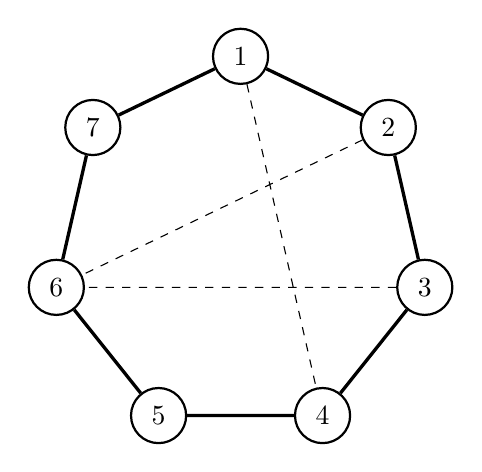
\begin{tikzpicture}[
  every node/.style={circle,draw,thick,minimum size=7mm,font=},
  ciclo/.style={very thick,black},
  cuerda/.style={black,dashed}]
  \foreach \v [count=\i from 0] in {1,...,7}
    \node (\v) at ({90-\i*360/7}:2.4) {\v};
  \draw[ciclo] (1)--(2)--(3)--(4)--(5)--(6)--(7)--(1);
  \draw[cuerda] (1)--(4) (2)--(6) (3)--(6);
\end{tikzpicture}
\caption{Grafo de ejemplo con $n=7$ y $m=10$. En azul, el único ciclo hamiltoniano; en
gris discontinuo, las tres aristas «trampa» $\{1,4\}$, $\{2,6\}$ y $\{3,6\}$.}
\label{aco:fig:ejemplo}
\end{figure}

\paragraph{Representación.} Lista de adyacencia:
$1\!:\!\{2,4,7\}$, $2\!:\!\{1,3,6\}$, $3\!:\!\{2,4,6\}$, $4\!:\!\{1,3,5\}$, $5\!:\!\{4,6\}$,
$6\!:\!\{2,3,5,7\}$, $7\!:\!\{1,6\}$.

\paragraph{Razonamiento estructural.} Los vértices 5 y 7 tienen grado 2, así que las aristas
$\{4,5\}$, $\{5,6\}$, $\{6,7\}$ y $\{7,1\}$ son obligatorias. Entonces el vértice 6 ya usa dos aristas
(hacia 5 y 7) y quedan descartadas $\{2,6\}$ y $\{3,6\}$. Falta unir 1 con 4 pasando por 2 y
3: solo es posible como $1\!-\!2\!-\!3\!-\!4$. El ciclo hamiltoniano es único:
$1\!-\!2\!-\!3\!-\!4\!-\!5\!-\!6\!-\!7\!-\!1$ (lo confirmamos enumerando las $6!$
permutaciones que empiezan en 1: solo esta y su recorrido inverso tienen costo 0). Este es
el mismo tipo de estructura que vuelve difíciles a las instancias del FHCP: pocas aristas
correctas escondidas entre muchas tentadoras \cite{aco8}.

\paragraph{Costo de permutaciones (función de penalización).}
\begin{center}
\begin{adjustbox}{max width=\linewidth}
\begin{tabular}{@{}lcl@{}}
\toprule
Permutación & Aristas faltantes & Motivo \\
\midrule
$\cite{aco1,aco4,aco3,aco6,aco7,aco2,aco5}$ & 3 & faltan $\{7,2\}$, $\{2,5\}$ y el cierre $\{5,1\}$ \\
$\cite{aco2,aco3,aco4,aco1,aco7,aco6,aco5}$ & 1 & todas existen salvo el cierre $\{5,2\}$ \\
$\cite{aco1,aco2,aco3,aco4,aco5,aco6,aco7}$ & 0 & ciclo hamiltoniano \\
\bottomrule
\end{tabular}
\end{adjustbox}
\end{center}

\paragraph{Primer paso de una hormiga.} Parámetros $\alpha=1$, $\beta=2$, $\tau_0=1$ en
todas las aristas y la heurística de Warnsdorff. Desde el vértice 1, los vecinos libres de
2, 4 y 7 son 2, 2 y 1, respectivamente, así que $\eta=(\tfrac12,\tfrac12,1)$ y
\[
  p_{12}=\frac{0.25}{0.25+0.25+1}=0.167,\quad p_{14}=0.167,\quad p_{17}=0.667.
\]
La heurística empuja hacia el vértice 7, de grado 2, que es correcto. Desde 7 el único
vecino libre es 6. En 6 (visitados $\{1,7,6\}$) los candidatos son 2, 3 y 5 con
$\eta=(1,\tfrac12,1)$, de modo que $p_{62}=0.444$, $p_{63}=0.111$, $p_{65}=0.444$.

\paragraph{Tres hormigas de la primera iteración.}
\begin{itemize}[nosep]
  \item Hormiga A: $1\!-\!7\!-\!6\!-\!2\!-\!3\!-\!4\!-\!5$. Visita los 7 vértices,
        pero $\{5,1\}$ no existe: camino hamiltoniano sin cierre. 6 aristas válidas.
  \item Hormiga B: $1\!-\!4\!-\!3\!-\!6\!-\!7$. En 7 sus vecinos (1 y 6) ya fueron
        visitados y faltan 2 y 5: callejón sin salida. 4 aristas válidas.
  \item Hormiga C: $1\!-\!7\!-\!6\!-\!5\!-\!4\!-\!3\!-\!2\!-\!1$. Ciclo
        hamiltoniano: 7 aristas válidas y cierre correcto.
\end{itemize}
Comprobación de C: longitud 7, sin repetidos, las aristas
$\{1,7\},\{7,6\},\{6,5\},\{5,4\},\{4,3\},\{3,2\}$ existen y el cierre $\{2,1\}$ también.

\paragraph{Actualización de feromonas} con $\rho=0.5$ y depósito
$\Delta\tau=(\text{aristas válidas})/n$: A deposita $6/7=0.857$, B $4/7=0.571$ y C $1$.

\begin{center}
\begin{adjustbox}{max width=\linewidth}
\begin{tabular}{@{}lcccccccccc@{}}
\toprule
Arista & 1-2 & 1-4 & 1-7 & 2-3 & 2-6 & 3-4 & 3-6 & 4-5 & 5-6 & 6-7 \\
\midrule
$\tau$ nueva & 1.500 & 1.071 & 2.357 & 2.357 & 1.357 & 2.929 & 1.071 & 2.357 & 1.500 & 2.929 \\
\bottomrule
\end{tabular}
\end{adjustbox}
\end{center}

En la segunda iteración, desde 6 (tras $1\!-\!7$) las probabilidades pasan a
$p_{62}=0.434$, $p_{63}=0.086$, $p_{65}=0.480$: el aprendizaje favorece la arista correcta,
pero lentamente, porque la hormiga A también reforzó la trampa $\{2,6\}$. Si se usa un
esquema elitista como MMAS, en el que solo deposita la mejor ruta (C), entonces
$\tau_{62}=0.5$, $\tau_{63}=0.5$ y $\tau_{65}=1.5$, y las probabilidades quedan en
$0.235$, $0.059$ y $0.706$. Lección: en grafos engañosos importa mucho quién
deposita feromona.

% =====================================================================
\section{Pseudocódigo y ajustes principales}
% =====================================================================

\begin{algorithm}[H]
\caption{ACO para el ciclo hamiltoniano (variante estilo MMAS)}
\label{aco:alg:aco}
\begin{algorithmic}[1]
\Require Grafo $G=(V,E)$ como listas de adyacencia; parámetros $m,\alpha,\beta,\rho,
         \tau_{\min},\tau_{\max}$, límite de iteraciones $T$
\Ensure Arreglo de $n$ vértices que forma un ciclo hamiltoniano, o la mejor ruta parcial
\State $\tau_{ij}\gets\tau_{\max}$ para toda $\{i,j\}\in E$
\State $\mathit{mejor}\gets$ ruta vacía
\For{$t=1$ to $T$}
  \For{$k=1$ to $m$}
    \State elegir vértice inicial $s$ al azar; $R_k\gets[s]$; $\mathit{visitados}\gets\{s\}$
    \While{$|R_k|<n$}
      \State $i\gets$ último vértice de $R_k$
      \State $N\gets$ vecinos de $i$ no visitados
      \If{$N=\emptyset$}
        \State intentar reparar con rotación de Pósa; si no se puede, break
      \Else
        \State elegir $j\in N$ con probabilidad $\propto\tau_{ij}^{\alpha}\eta_{ij}^{\beta}$
        \State añadir $j$ a $R_k$ y a $\mathit{visitados}$
      \EndIf
    \EndWhile
    \State $q_k\gets$ (aristas válidas de $R_k$, incluido el cierre si existe)$/n$
    \If{$q_k=1$ y $R_k$ pasa el verificador completo} \Return $R_k$ \Comment{ciclo hamiltoniano encontrado}
    \EndIf
    \If{$q_k>$ calidad de $\mathit{mejor}$} $\mathit{mejor}\gets R_k$
    \EndIf
  \EndFor
  \State $\tau_{ij}\gets(1-\rho)\tau_{ij}$ para toda arista \Comment{evaporación}
  \State $\tau_{ij}\gets\tau_{ij}+q_{\mathit{mejor}}$ para cada arista de $\mathit{mejor}$
         \Comment{depósito}
  \State acotar $\tau_{ij}$ al intervalo $[\tau_{\min},\tau_{\max}]$
\EndFor
\State \Return $\mathit{mejor}$
\end{algorithmic}
\end{algorithm}

\begin{table}[H]
\centering
\caption{Ajustes principales y valores de partida. Los valores de referencia son los que
Dorigo y Stützle \cite{aco3} recomiendan para el TSP; hay que calibrarlos para el FHCP.}
\label{aco:tab:params}
\begin{adjustbox}{max width=\linewidth}
\begin{tabular}{@{}p{2.7cm}p{6.9cm}p{4.4cm}@{}}
\toprule
Parámetro & Efecto & Referencia (TSP) \\
\midrule
$m$ (hormigas) & Más hormigas exploran más por iteración, pero cuestan más tiempo.
               & $m=n$ (AS, MMAS); $m=10$ (ACS) \\
$\alpha$ & Peso de la feromona (lo aprendido). Muy alto: convergencia prematura. & $1$ \\
$\beta$  & Peso de la heurística (la estructura del grafo). & $2$ a $5$ \\
$\rho$   & Evaporación. Alta: olvida rápido y explora; baja: explota lo aprendido.
         & $0.5$ (AS), $0.1$ (ACS), $0.02$ (MMAS) \\
$\tau_{\min},\tau_{\max}$ & Evitan que una arista quede con probabilidad casi 0 o casi 1. & MMAS \\
$q_0$    & (ACS) probabilidad de elegir directamente el mejor vecino. & $0.9$ \\
$T$      & Límite de iteraciones o de tiempo; necesario para la comparación. & ---\\
\bottomrule
\end{tabular}
\end{adjustbox}
\end{table}

% =====================================================================
\section{Aplicación al ciclo hamiltoniano: opciones, dificultades y dudas}
% =====================================================================

\subsection{Opciones de diseño}
\begin{enumerate}
  \item \prop{} Grafo de construcción = grafo del problema: las hormigas solo se
        mueven por aristas reales, así que no repiten vértices ni recorren aristas inexistentes; las fallas se
        reducen a «no llegó a todos» o «no cerró».
  \item \prop{} Calidad = fracción de aristas válidas. Es equivalente a
        $1-f(\pi)/n$ con la función de penalización presentada en este capítulo, para permutaciones completas. En rutas parciales, esta puntuación es solo una guía interna; la comparación entre métodos debe usar éxito verificado y presupuesto.
  \item \prop{} Variante MMAS o ACS: el ejemplo muestra que el depósito de todas las
        hormigas refuerza trampas; un esquema elitista con límites de feromona es más
        apropiado.
  \item \prop{} Preprocesamiento: fijar las aristas obligatorias de los vértices de
        grado 2 antes de lanzar la colonia.
  \item \prop{} Búsqueda local: combinar ACO con rotaciones de Pósa o 2-opt
        restringido a aristas existentes, como se hace con ACO+búsqueda local en el TSP \cite{aco3}.
\end{enumerate}

\subsection{Dificultades previstas}
\begin{itemize}[nosep]
  \item Las instancias del FHCP están construidas para engañar a heurísticas estándar \cite{aco8};
        muchas aristas «atractivas» no pertenecen a ningún ciclo.
  \item Si el número de hormigas es $m=n$ y el grafo tiene miles de vértices, una iteración
        cuesta del orden de $n^2$ pasos; para $n\approx9500$ son unos $9\times10^7$ pasos.
  \item La feromona mide aristas, pero el problema es global: una arista puede estar en
        rutas casi completas y aun así no pertenecer a ningún ciclo hamiltoniano.
  \item Las rutas que fallan muy pronto dan poca información; la retroalimentación es escasa.
  \item Como referencia de dificultad, el ganador del concurso FHCP resolvió 985 de las
        1001 instancias \cite{aco9}; no se espera que una metaheurística simple las resuelva todas.
\end{itemize}

\subsection{Dudas pendientes}
\begin{enumerate}[nosep]
  \item \duda{} ¿El profesor espera trabajar con las 1001 instancias o con un subconjunto
        (por ejemplo, las más pequeñas)?
  \item \duda{} ¿Qué límite de tiempo o de iteraciones usaremos para que la comparación sea
        justa entre los seis algoritmos?
  \item \duda{} ¿Se permite combinar ACO con búsqueda local o reparación, o se pide la
        versión «pura» del algoritmo?
  \item \duda{} ¿Cómo aplicar precisión, recall y F1 (tema del integrante 4) a un
        problema donde todas las instancias son hamiltonianas? Una propuesta es tratar
        «encontró el ciclo» como predicción positiva y comparar contra la solución oficial.
  \item \duda{} ¿Acordamos en el equipo una única función de costo (aristas faltantes) para
        todos los algoritmos?
\end{enumerate}

% =====================================================================
